\documentclass[12pt,a4paper,twocolumn]{article}
\usepackage[T1]{fontenc}
\usepackage[utf8]{inputenc}
\usepackage[ngerman]{babel}
\usepackage[a4paper,top=26mm,left=26mm,right=26mm,bottom=28mm]{geometry}
\usepackage{newtxtext,newtxmath}
\usepackage[protrusion=false]{microtype}
\usepackage{amsmath}
\usepackage{booktabs}
\usepackage{array}
\usepackage{graphicx}
\usepackage{float}
\usepackage{balance}
\usepackage{caption}
\usepackage{titlesec}
\usepackage{fancyhdr}
\usepackage{enumitem}
\usepackage{xcolor}
\usepackage[hidelinks,pdfusetitle]{hyperref}
\usepackage{xurl}

\definecolor{resultblue}{HTML}{176B87}
\definecolor{softblue}{HTML}{EAF2F5}
\definecolor{rulegray}{HTML}{64707A}

\setlength{\baselineskip}{14.4pt}
\setlength{\parindent}{1.25em}
\setlength{\parskip}{0pt}
\setlength{\columnsep}{8mm}
\setlength{\emergencystretch}{5em}
\sloppy
\renewcommand{\footnotesize}{\fontsize{12}{14.4}\selectfont}
\renewcommand{\small}{\fontsize{12}{14.4}\selectfont}
\renewcommand{\arraystretch}{1.12}
\setlist{nosep,leftmargin=1.4em}

\titleformat{\section}{\raggedright\hyphenpenalty=10000\fontsize{14}{16.8}\selectfont\bfseries}{\thesection.}{0.5em}{}
\titleformat{\subsection}{\raggedright\hyphenpenalty=10000\fontsize{12}{14.4}\selectfont\bfseries}{\thesubsection.}{0.5em}{}
\titlespacing*{\section}{0pt}{10pt}{5pt}
\titlespacing*{\subsection}{0pt}{8pt}{4pt}

\captionsetup{font=normalsize,labelfont=bf,labelsep=period,singlelinecheck=false,skip=4pt}
\captionsetup[table]{position=below}

\pagestyle{fancy}
\fancyhf{}
\fancyfoot[C]{\raisebox{7mm}[0pt][0pt]{\thepage}}
\renewcommand{\headrulewidth}{0pt}
\setlength{\footskip}{6mm}

\newcommand{\sourcecaption}[1]{\par\vspace{2pt}{\fontsize{12}{14.4}\selectfont #1\par}}
\newcommand{\E}{\mathrm{e}}
\newcommand{\dd}{\mathrm{d}}
\newcommand{\Unit}[1]{\,\mathrm{#1}}
\newcommand{\QFinal}{877.8}
\newcommand{\QFinalFull}{877.781}
\newcommand{\KDurchfluss}{9.646}
\newcommand{\QDry}{578.8}
\newcommand{\QChiller}{299.0}
\newcommand{\PElectric}{74.2}
\newcommand{\EElectric}{650.1}
\newcommand{\PChiller}{59.805}
\newcommand{\PFans}{14.064}
\newcommand{\PPumps}{0.338}
\newcommand{\EnergyCostFinal}{116.36}
\newcommand{\MaintenanceFinal}{21.58}
\newcommand{\QCondenser}{358.8}
\newcommand{\QAirRejection}{952.0}
\newcommand{\QFloodStress}{12.48}
\newcommand{\BufferVolume}{8280}
\newcommand{\PipeDiameter}{0.70}
\newcommand{\QReserve}{1053.3}
\newcommand{\QModule}{175.6}
\newcommand{\QStorage}{0.0303}
\newcommand{\EvapRate}{358.3}
\newcommand{\EvapAnnual}{11.30}
\newcommand{\EvapFraction}{15.6}
\newcommand{\DilutionFlow}{52.3}
\newcommand{\DilutionRatio}{22.8}
\newcommand{\PassiveArea}{4.4}
\newcommand{\CapexFinal}{719}
\newcommand{\OpexFinal}{137.9}
\newcommand{\NpvHybrid}{2.90}
\newcommand{\NpvUpfront}{3.01}
\newcommand{\NpvSaving}{112}
\newcommand{\NpvEvap}{0.78}
\newcommand{\NpvDilution}{11.48}
\newcommand{\FailureMinutes}{23}
\newcommand{\PoolTau}{3.02}
\newcommand{\QSampleLow}{480}
\newcommand{\QSampleHigh}{1528}
\newcommand{\NpvSampleLow}{2.36}
\newcommand{\NpvSampleHigh}{3.81}


\hypersetup{pdftitle={Blautopf dauerhaft vor dem Sieden bewahren},pdfauthor={},pdfsubject={PlaNeT SimTech Szenariobericht},pdfkeywords={}}

\begin{document}

\begin{titlepage}
  \centering
  \vspace*{24mm}
  {\fontsize{16}{20}\selectfont PlaNeT SimTech\par}
  \vspace{14mm}
  {\fontsize{22}{27}\selectfont\bfseries Blautopf dauerhaft vor dem Sieden bewahren\par}
  \vspace{8mm}
  {\fontsize{14}{18}\selectfont Szenariobericht mit Auslegung, Alternativenprüfung und Unsicherheitsanalyse\par}
  \vspace{18mm}
  {\fontsize{12}{15}\selectfont\bfseries Aufgabenstellung\par}
  \vspace{3mm}
  Wie kann dauerhaft verhindert werden, dass das Wasser im Blautopf den Siedepunkt erreicht?
  \vfill
  Team-ID: TEST-K31pro-max\par
  \vspace{3mm}
  Datum: 07.11.2026\par
  \vspace{10mm}
  Vulkanische Tiefenerwärmung und die Zehnjahresprognose sind Vorgaben des Szenarios. Sie sind keine durch diesen Bericht bestätigten Beobachtungen.
  \vspace{8mm}
\end{titlepage}

\setcounter{page}{1}
\section*{Zusammenfassung}

Der Blautopf ließe sich im vorgegebenen Szenario dauerhaft vor dem Sieden schützen, indem der gesamte betroffene Quellstrom vor dem offenen Becken gekühlt wird. Große Luftkühler nutzen zuerst die hohe Temperaturdifferenz. Danach senken Kältemaschinen das Wasser auf etwa 9 °C. Ein Mischbecken begrenzt die Temperaturänderung am ökologischen Kontrollpunkt auf höchstens 1 °C pro Stunde. Die Wärme darf nicht in denselben Wasserkreislauf zurückkehren.

Die Aufgabe ist vor allem eine Frage der Größe. Im zehnten Jahr müsste die Anlage \textbf{\QFinal\ Megawatt Wärme abführen}. Diese Zahl folgt aus 2,3 Kubikmetern Wasser pro Sekunde, die von 100 auf 9 °C abgekühlt werden. Eine Rechnung, die nur das angenommene Beckenvolumen erwärmt, ergibt dagegen \QStorage\ Megawatt. Sie übersieht den ständigen Zufluss und taugt nicht zur Auslegung.

Der Entwurf besitzt in jeder Ausbaustufe sechs getrennte Stränge. Fünf tragen die Last, der sechste ist Reserve. Im Endausbau sind \QReserve\ Megawatt installiert. Ein Puffer von \BufferVolume\ Kubikmetern entspricht einer Stunde mittleren Quellstroms. Notstrom, Ersatzmodule und unabhängige Temperatur- und Druckmessungen sind nötig, weil ein Speicher bei einem Ausfall keine dauerhafte Sicherheit bietet.

Die geschlossene Bauweise ist teuer, erhält aber den Wasserhaushalt. Die Szenarioschätzung ergibt \textbf{\CapexFinal\ Millionen Euro Investition} und rund \OpexFinal\ Millionen Euro Betriebskosten im zehnten Jahr. Die über 25 Jahre abgezinsten Gesamtkosten betragen \NpvHybrid\ Milliarden Euro. Verdunstungskühlung wäre billiger, würde aber jährlich \EvapAnnual\ Millionen Kubikmeter Wasser verbrauchen und zusätzliche Hygienepflichten auslösen. Kaltwasserzumischung bräuchte eine nicht nachgewiesene Wasserquelle mit mehr als dem Zwanzigfachen des natürlichen Quellstroms.

Die Lösung gilt nur innerhalb einer klaren Hülle. Höchstens 2,3 Kubikmeter pro Sekunde sind von der Erwärmung betroffen. Ihre Temperatur steigt binnen zehn Jahren von 9 auf 100 °C und bleibt danach höchstens dort. Ein vollständig erwärmter Hochwasserstrom würde \QFloodStress\ Gigawatt Kühlung verlangen und ist nicht abgedeckt. Vor einem Bau müssen Messungen zeigen, welcher Karstast wie viel Wärme führt. Alle Kosten sind Schätzungen in Euro von 2026, keine Angebote. Eine Genehmigung, menschliche Prüfung oder tatsächliche Einreichung wird nicht behauptet.

\section{Einführung: Die Wärme ist das Problem}

Wenn Dampf über dem Blautopf stünde, wäre das eigentliche Ziel bereits verfehlt. Sieden ist die späte physikalische Grenze. Für Organismen können weit niedrigere Temperaturen und auch ein zu schnelles Abkühlen schädlich sein [9,10]. Die Antwort muss deshalb mehr leisten als eine Abdeckung, die Dampfblasen verbirgt, oder ein höherer Druck, der das Sieden erst bei höherer Temperatur eintreten lässt. Die zugeführte Wärme muss das verbundene Wassersystem verlassen.

Der Blautopf entwässert einen Karstaquifer von etwa 165 km². Zwei verbundene Höhlenäste, Ur-Blau und Nord-Blau, sind bekannt. Die bekannte Systemlänge von etwa 15,5 km ist keine vollständige Länge des unterirdischen Strömungsnetzes [3]. Tracerversuche zeigen unterschiedliche Strömungsbereiche und Fließgeschwindigkeiten [11]. Eine Anlage, die nur eine bequem zugängliche Stelle kühlt, könnte deshalb den Wärmeträger verfehlen.

Gleichzeitig ist der Quellstrom gut dokumentiert. Für 1952 bis 2021 beträgt der mittlere Abfluss 2,3 m³/s, die Quantile für 10 und 90 Prozent liegen bei 0,7 und 4,7 m³/s [2]. Gerade dieser Durchfluss macht die Aufgabe anspruchsvoll. Er transportiert pro Kelvin Temperaturdifferenz etwa 9,65 Megawatt. Ein kleiner Kältekreislauf an einem Teilstrom kann deshalb nur dann genügen, wenn Messungen beweisen, dass auch nur dieser kleine Teilstrom die Anomalie trägt.

Dieser Bericht vergleicht sieben unabhängig abgeleitete Ansätze mit denselben physikalischen Regeln. Er wählt die hybride Vollstromkühlung H1, rechnet ihre Wärme- und Kostenbilanz und benennt Beobachtungen, die Entwurf oder Erfolg widerlegen würden. Die vulkanische Ursache und die Zehnjahresprognose bleiben Szenariovorgaben. Die zitierten Fachquellen belegen weder vulkanische Aktivität am Blautopf noch eine solche Prognose. Anhang A dokumentiert die umfassende KI-Nutzung und die Unabhängigkeit der Herleitung.

\section{Methode, Daten und Annahmen}

\subsection{Messdaten und Szenarioannahmen}

Die belastbarste Ausgangsgröße ist der Abfluss. Fan, Goeppert und Goldscheider werteten die LUBW-Station 76273 über 1952 bis 2021 aus. Sie berichten neben dem Mittelwert tägliche Werte von 0,1 bis 32,6 m³/s [2]. Das Landesamt für Geologie, Rohstoffe und Bergbau nennt für einen anderen Zeitraum und eine andere Statistik einen Hochwasserwert von 32,7 m³/s [3]. Diese Zahlen sind nicht austauschbar. Der Bericht verwendet 2,3 m³/s als Referenzstrom und 32,7 m³/s ausschließlich als separaten Stresstest.

\begin{table}[H]
\centering
\begin{tabular}{@{}>{\hspace{0pt}\raggedright\arraybackslash}p{22mm}>{\hspace{0pt}\raggedright\arraybackslash}p{16mm}>{\hspace{0pt}\raggedright\arraybackslash}p{24mm}@{}}
\toprule
Größe & Wert & Status und Herkunft \\
\midrule
Mittlerer Abfluss & 2,3 m³/s & Messreihe [2] \\
Abflussquantile & 0,7 und 4,7 m³/s & 10- und 90-Prozent-Quantil [2] \\
Beckentiefe & 20,6 bis 22 m & keine neue Vermessung [1,3] \\
Ausgangstemperatur & etwa 9 °C & öffentliche Angabe [1] \\
Tiefenerwärmung & 9 auf 100 °C & linear in zehn Jahren, Szenario \\
Temperatur danach & höchstens 100 °C & Entwurfsgrenze \\
Betroffener Strom & höchstens 2,3 m³/s & Entwurfsannahme \\
Beckenvolumen & 25.000 m³ & Rechenannahme, keine Bathymetrie \\
Auslegungsluft & 35 °C & technische Annahme \\
Rückführziel & 9 °C, 1 K/h & ökologisches Regelziel [1,10] \\
\bottomrule
\end{tabular}
\caption{Tabelle 1 trennt Messwerte, Szenarioprämissen und technische Annahmen.}
\end{table}

Die 9 °C der Stadt eignen sich als Ausgangswert, aber nicht als Ersatz für eine mehrjährige Temperaturmessung [1]. Ebenso fehlen aktuelle Beckenvermessung, vertikale Temperaturprofile, Astabflüsse und eine lokale Wärmebilanz der Wasseroberfläche. Diese Lücken werden nicht durch scheinbar genaue Nachkommastellen verdeckt.

\subsection{Wärme- und Druckbilanz}

Für Wasser ohne Phasenwechsel gilt die sensible Wärmeleistung
\begin{equation}
\dot Q=\rho\,\dot V\,c_p\,(T_{ein}-T_{ziel}).
\label{eq:sensible}
\end{equation}
Dabei sind \(\rho\) die Dichte, \(\dot V\) der betroffene Volumenstrom und \(c_p\) die spezifische Wärmekapazität. Die Gleichung folgt aus der Energieerhaltung und ist Bestandteil allgemeiner Wasser- und Wärmebilanzen [6,7]. Die Rechnung verwendet \(\rho=999,702\ \mathrm{kg/m^3}\) und \(c_p=4195,14\ \mathrm{J/(kg\,K)}\) aus der NIST-Tabelle bei etwa 10 °C und 1,01325 bar [4]. Über den gesamten Temperaturpfad konstante Stoffwerte sind eine Näherung. Für eine spätere Detailauslegung sind temperatur- und druckabhängige IAPWS-Werte erforderlich [5].

Mit dem Mittelstrom ergibt sich der Wärmekapazitätsstrom
\begin{equation}
C=\rho\,\dot V\,c_p=\KDurchfluss\ \mathrm{MW/K}.
\label{eq:capacity}
\end{equation}
Das Szenario bildet die Tiefentemperatur als
\begin{equation}
T_q(t)=\min(9+9,1t,100),\quad t\ \text{in Jahren},
\end{equation}
ab. Die jährlich benötigte Kühlung ist \(C\,[T_q(t)-9]\) für positive Differenzen. Oberflächen- und Sohlverluste werden nicht als Gegenleistung angerechnet, weil Flächen, Windfunktion und lokale Austauschkoeffizienten unbekannt sind. Die allgemeine Flussenergiebilanz enthält Strahlung, Verdunstung, fühlbare Wärme und Sohlaustausch [6]. Diese Terme können die Rechnung später verbessern, werden hier aber nicht mit erfundenen Standortwerten gefüllt.

Zusätzlich muss an jedem Ort und zu jeder Zeit die Siedebedingung
\begin{equation}
T+u_T<T_{sat}(p_{abs})-\Delta T_S
\label{eq:boiling}
\end{equation}
gelten. Dabei ist \(u_T\) die Mess- und Modellunsicherheit, \(\Delta T_S\) eine noch mit der Behörde festzulegende Sicherheitsmarge. Der Siedepunkt hängt vom absoluten Druck ab [5]. Eine Oberflächenmessung allein beweist daher nicht, dass Tiefe, Steigleitung und Rückführung sicher bleiben.

\subsection{Vergleichs- und Kostenregeln}

Jeder Ansatz muss die gesamte Wärmebilanz schließen, bei 35 °C Außenluft auf 9 °C kühlen können und die Wärme außerhalb des verbundenen Grund- und Oberflächenwassers abgeben. Eine Umleitung, die das Becken selbst weiter erwärmt, oder eine bloße Erhöhung des Siedepunkts scheidet vor dem Kostenvergleich aus. Erst danach entscheiden Wasserbedarf, Umweltfolgen, Betriebssicherheit und Kosten.

Alle Geldbeträge sind Szenarioschätzungen in Euro von 2026. Der Barwert über 25 Jahre lautet
\begin{equation}
K_0=\sum_{y=0}^{25}\frac{I_y+B_y+M_y+E_y}{(1+0,03)^y}.
\label{eq:npv}
\end{equation}
Hier sind \(I_y\) Investitionen, \(B_y\) Strom, Wasser und Hygiene abzüglich Wärmeerlösen, \(M_y\) Wartung und \(E_y\) Ersatzinvestitionen. Die Wartung beträgt jährlich 3 \% der installierten Investition. In Jahr 15 werden 25 \% der variablen Endausrüstung ersetzt. Der Strompreis beträgt 179 €/MWh, passend zum ausgewiesenen Preis von 17,9 ct/kWh für kleine und mittlere Industrie [16]. Für Wasser werden 0,50 €/m³ und für die Hygiene von H2 0,5 Mio. € pro Jahr angesetzt. Wärmeerlöse bleiben im Referenzfall null.

Der Stückpreis von 15 €/kW für Wärmetauscher orientiert sich am oberen Listenpreis eines einzelnen Plattenapparats, nicht an einer Anlage am Blautopf [18]. Kältemaschinen mit 500 €/kW, Trockenkühler mit 120 €/kW, Tiefbau, Steuerung, Notstrom und Zuschläge sind ausdrücklich Modellannahmen. Auf die variable Ausrüstung werden 20 \% Leistungsreserve und anschließend 60 \% Zuschlag für Engineering und Unvorhergesehenes gerechnet. Es gibt weder standortbezogene Geräteangebote noch Ausschreibungsergebnisse. Historische Kostenliteratur dient nur als weiterer Anker [19].

\section{Ergebnisse}

\subsection{Vollstrom und Speicher unterscheiden sich um vier Größenordnungen}

Im zehnten Jahr beträgt die Temperaturdifferenz 91 K. Die erforderliche Wärmeabfuhr ist daher
\begin{equation}
\dot Q_{10}=C(100-9)=\QFinalFull\ \mathrm{MW}.
\label{eq:qfinal}
\end{equation}
Diese Zahl enthält noch keine Verdampfung des gesamten Wassers. Sie beschreibt allein die Abkühlung von 100 auf 9 °C. Die volle Anlage muss diese Leistung dauerhaft abführen, solange der heiße Zufluss fortdauert.

Die kleine Speichergrenze entsteht aus einer anderen Frage. Welche durchschnittliche Leistung würde ein abgeschlossenes, angenommenes Beckenvolumen von 25.000 m³ innerhalb von zehn Jahren von 9 auf 100 °C erwärmen? Mit einem Modelljahr von 8760 Stunden gilt
\begin{equation}
\dot Q_V=\frac{\rho Vc_p(100-9)}{10\cdot365\cdot86400}
=\QStorage\ \mathrm{MW}.
\end{equation}
Der Vollstromfall ist rund 29.000-mal größer. Die Speichergrenze ignoriert, dass bei 2,3 m³/s das angenommene Beckenvolumen rechnerisch alle \PoolTau\ Stunden ersetzt wird. Als alleinige Auslegungsgrundlage würde sie die dauerhafte Wärmezufuhr unterschätzen. Umgekehrt ist der Vollstromwert keine Messung der vulkanischen Leistung. Er ist die notwendige Kühlleistung unter der ausdrücklichen Annahme, dass der gesamte Mittelstrom mit 100 °C ankommt.

\begin{figure*}[t]
\centering
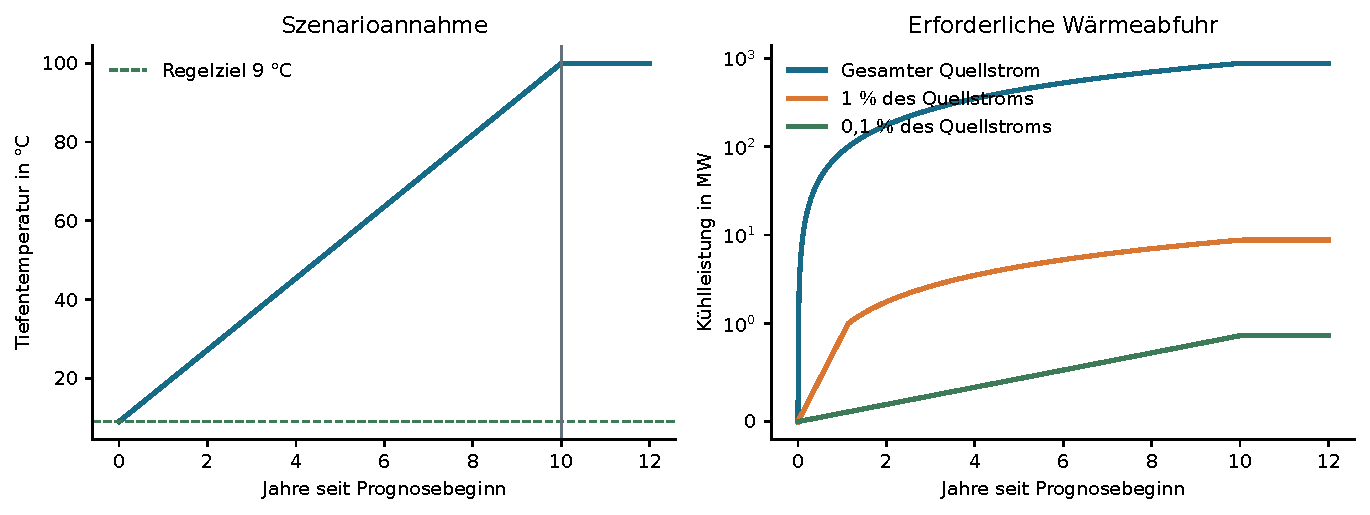
\includegraphics[width=\textwidth]{figures/fig01_prognose_last.pdf}
\caption{Abbildung 1 zeigt die Szenariotemperatur und die daraus folgende Kühlleistung. Der Maßstab hängt entscheidend davon ab, welcher Anteil des Quellstroms die Anomalie trägt. Eigene Darstellung mit Python und Kimi K3.1 Pro aus [2,4].}
\label{fig:prognose}
\end{figure*}

\subsection{Trockenkühlung und Kältemaschinen teilen die Last}

Bei 35 °C Außenluft und einer angenommenen Annäherung von 5 K kann die direkte Trockenkühlung das heiße Wasser im Auslegungsjahr auf 40 °C bringen. Sie übernimmt
\begin{equation}
\dot Q_{trocken}=C(100-40)=\QDry\ \mathrm{MW}.
\end{equation}
Erst die zweite Stufe kühlt von 40 auf 9 °C:
\begin{equation}
\dot Q_{K}=C(40-9)=\QChiller\ \mathrm{MW}.
\end{equation}
Damit ist H1 keine kleine Wärmepumpe mit einem symbolischen Teilstrom. Die Anlage erfasst den vollen mittleren Quellstrom und kombiniert \QDry\ MW direkte Kühlung mit \QChiller\ MW Kältemaschinenkühlung. In kühleren Jahren übernehmen die Kältemaschinen einen größeren Anteil, weil die Trockenkühler unterhalb ihrer Annäherungstemperatur nicht weiter kühlen können.

Für die Kältemaschinen gilt \(COP_C=\dot Q_K/W_K\) und \(\dot Q_{Kond}=\dot Q_K+W_K\) [8]. Der verwendete \(COP_C=5\) ist eine Szenarioannahme, keine Herstellerkurve. Feldmessungen an Grundwasser-Wärmepumpen weisen Jahresarbeitszahlen von 2,33 bis 4,76 aus, weshalb die Sensitivität den Bereich 3,0 bis 6,5 umfasst [17]. Beim Referenzwert beträgt die elektrische Leistung \PChiller\ MW. Die Kondensatoren müssen deshalb
\begin{equation}
\dot Q_{Kond}=299,024+59,805=\QCondenser\ \mathrm{MW}
\end{equation}
abgeben. Diese Wärme ist größer als die von den Kältemaschinen entzogene Wärme, weil die elektrische Antriebsenergie ebenfalls als Wärme anfällt. Wer nur die 299 MW nennt, unterschlägt einen wesentlichen Teil der Wärmesenke.

Mit 1,5 \% Ventilatorhilfsleistung auf Trocken- und Kondensatorkühlung sowie \PPumps\ MW Pumpenleistung ergibt sich
\begin{equation}
P_{el}=\PChiller+\PFans+\PPumps=\PElectric\ \mathrm{MW}.
\end{equation}
Die vollständige externe Wärmesenke beträgt folglich
\begin{equation}
\dot Q_{Senke}=\dot Q_{10}+P_{el}=\QAirRejection\ \mathrm{MW}.
\end{equation}
Die Anlage muss also \QAirRejection\ MW an Luft oder an nachgewiesene externe Wärmeabnehmer abgeben. Eine Rückführung in Blau, Blautopf oder denselben Aquifer würde die Bilanz aufheben und zusätzlich die Antriebsenergie eintragen [8]. Flächenbedarf, Luftführung, Rückverwirbelung, Geräusche und lokale Erwärmung sind noch nicht standortbezogen untersucht. Die geschlossene Bilanz beweist die Energieerhaltung, nicht die bauliche Machbarkeit an diesem Ort.

\subsection{Module, Puffer und Notstrom sichern den Betrieb}

Der Endausbau besitzt sechs thermisch gleiche Stränge. Fünf Stränge mit je \QModule\ MW decken die \QFinal\ MW Last. Der sechste Strang bildet die N+1-Reserve. Installiert sind damit \QReserve\ MW, also 20 \% mehr als benötigt. Jedes lasttragende Modul führt etwa 0,46 m³/s. Bei einer angenommenen Rohrgeschwindigkeit von 1,2 m/s folgt
\begin{equation}
d=\sqrt{\frac{4\cdot0,46}{\pi\cdot1,2}}=\PipeDiameter\ \mathrm{m}.
\end{equation}
Dies ist ein hydraulischer Richtwert, noch keine Rohrklasse oder Druckauslegung. Die Entnahme erfolgt geschlossen und druckgehalten, bevor heißes Wasser bei fallendem Druck seinen lokalen Siedepunkt erreichen kann. Als hydrostatisches Beispiel ergeben 22 m Wassertiefe 3,17007 bar absoluten Druck und einen Sättigungspunkt von 135,413 °C [4,5]. Dieses Beispiel ersetzt kein Druckprofil im Höhlennetz.

In jeder Ausbaustufe wird die benötigte Leistung auf fünf aktive und einen reservierten Strang verteilt. Frühe Module sind kleiner und werden erweitert oder ersetzt. Die Kostenrechnung enthält deshalb in jedem Jahr 20 \% Reserve. Jahr 0 umfasst Messinfrastruktur, Tiefbau und Steuerung mit 95 Mio. €. Im Modell steigt die benötigte Kühlung von 87,8 MW in Jahr 1 über 438,9 MW in Jahr 5 auf 877,8 MW in Jahr 10. Jede Stufe muss vor dem prognostizierten Lastjahr getestet sein. Der Stufenplan spart gegenüber dem sofortigen Endausbau \NpvSaving\ Mio. € Barwert, darf aber keine Sicherheitsstufe verzögern.

Ein externer Misch- und Pufferspeicher von
\begin{equation}
V_P=2,3\cdot3600=\BufferVolume\ \mathrm{m^3}
\end{equation}
fasst eine Stunde des Referenzstroms. Dort wird die Rückführung so geregelt, dass die Temperaturänderung am ökologischen Kontrollpunkt höchstens 1 K/h beträgt. Dieser Wert folgt einer LAWA-Empfehlung für schnelle Temperaturänderungen und wird hier als eigenes Regelziel verwendet, nicht als automatisch geltende Blau-Grenze [10]. Die konkrete OGewV-Typzuordnung der Blau und die behördlich anzulegenden Temperaturgrenzen sind nicht bestätigt [9]. Der Puffer glättet die Rückkehr. Er kühlt nicht dauerhaft und ersetzt weder Reservemodul noch Notstrom.

Für einen Stromausfall ist eine Ersatzstromversorgung für die volle erforderliche Antriebsleistung von \PElectric\ MW vorzusehen. Der Kostenschätzposten enthält dafür 60 Mio. €. Aggregatzahl, Brennstoffvorrat, Überbrückungsdauer und Netzschutz sind noch nicht ausgelegt. Die Dringlichkeit zeigt ein vereinfachter Ausfalltest: Bei 100 °C heißem Zufluss, 25.000 m³ ideal gemischtem Becken und vollständigem Kühlungsausfall gilt \(T(t)=100+(9-100)e^{-t/\tau}\) mit \(\tau=\PoolTau\) h. Bereits nach \FailureMinutes\ Minuten erreicht das Modell 20 °C. Das ist kein prognostizierter realer Temperaturverlauf, aber ein Argument für automatische Fehlererkennung, redundante Messketten und sofort verfügbare Reserveleistung.

\section{Alternativen und Wirtschaftlichkeit}

\subsection{H1, H2 und H3 im gleichen Kostenmodell}

Die folgende Tabelle verwendet identische Last, Laufzeit und Diskontierung. Die Investition enthält die jeweils modellierte Reserve. Die Betriebskosten beziehen sich auf Jahr 10 und enthalten keine neue Investition oder Ersatzinvestition. Alle Angaben sind Szenarioschätzungen in Euro von 2026.

\begin{table*}[t]
\centering
\begin{tabular}{@{}p{51mm}rrr@{}}
\toprule
Größe im Auslegungsjahr & H1 Hybrid & H2 Verdunstung & H3 Zumischung \\
\midrule
Wärmeabfuhr in MW & 877,8 & 877,8 & 877,8 \\
Investition in Mio. € & 719,4 & 283,9 & 119,6 \\
Elektrische Leistung in MW & 74,2 & 13,5 & 12,8 \\
Strom pro Jahr in GWh & 650,1 & 118,3 & 112,4 \\
Zusatzwasser pro Jahr & 0 m³ & 11,30 Mio. m³ & 1,650 Mrd. m³ \\
Betriebskosten in Mio. € & 137,9 & 35,8 & 848,8 \\
Barwert in Mrd. € & 2,897 & 0,780 & 11,478 \\
\bottomrule
\end{tabular}
\caption{Tabelle 2 vergleicht die drei dimensionierten Ansätze. H2 ist am günstigsten, verändert aber den Wasserhaushalt und das Hygieneregime.}
\end{table*}

Bei H1 setzen sich die jährlichen Betriebskosten aus \EnergyCostFinal\ Mio. € Strom und \MaintenanceFinal\ Mio. € Wartung zusammen. Der gestaffelte Barwert liegt bei \NpvHybrid\ Mrd. € gegenüber \NpvUpfront\ Mrd. € bei sofortigem Endausbau. Die Differenz ist ein Rechenvorteil des bedarfsgerechten Ausbaus, keine Erlaubnis für verspätete Sicherheitsreserve.

\begin{figure*}[t]
\centering
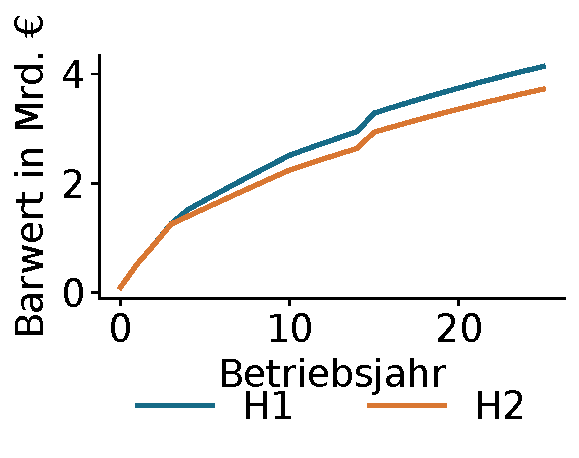
\includegraphics[width=\textwidth]{figures/fig03_kostenpfad.pdf}
\caption{Abbildung 2 zeigt die kumulierten Barwertkosten. H1 ist teurer, vermeidet aber den jährlichen Wasserverbrauch von H2. Eigene Rechnung mit Kimi K3.1 Pro.}
\label{fig:kosten}
\end{figure*}

H2 nutzt Verdunstungswärme. Mit einem Screeningwert von 2,45 MJ/kg folgt aus der vollen Last ein Wasserdampfstrom von \EvapRate\ kg/s [6]. Der jährliche Ersatzwasserbedarf beträgt \EvapAnnual\ Mio. m³. Bezogen auf das Quellsystem wären das \EvapFraction\ \% des mittleren Abflusses. Herkunft und ökologische Verträglichkeit dieses Wassers sind nicht nachgewiesen. Auch das 9-°C-Ziel ist bei warmer, feuchter Luft ohne gemessene Feuchtkugeltemperatur nicht garantiert. Offene Verdunstungssysteme unterliegen Anforderungen zu Bau, Betrieb, Kontrolle, Laboruntersuchung, Protokoll und Prüfung nach der 42. BImSchV [13]. Aerosole, Schaum und Sichtwirkung kommen als Prüffragen hinzu. H2 ist im Modell am billigsten, aber kein gleichwertiger Ersatz für den wasser- und hygieneärmaren H1.

H3 mischt 5 °C kaltes Wasser zu. Aus der Energiebilanz folgt
\begin{equation}
\begin{aligned}
\dot V_k&=\frac{877,781\cdot10^6}{999,702\cdot4195,14\cdot(9-5)}\\
&=\DilutionFlow\ \mathrm{m^3/s}.
\end{aligned}
\end{equation}
Das ist das \DilutionRatio-fache des natürlichen Mittelstroms als zusätzlicher Kaltwasserstrom. Die Mischung würde den Abfluss auf 54,625 m³/s erhöhen. Eine ganzjährig verfügbare, kalte und ökologisch verträgliche Quelle dieser Größe ist nicht belegt. Allein der angesetzte Wasserpreis erzeugt 825,06 Mio. € der jährlichen Betriebskosten. H3 scheidet deshalb trotz einfacher Technik aus.

H1 kostet bewusst mehr als H2. Der Aufpreis kauft einen geschlossenen Prozess ohne modellierten jährlichen Wasserverbrauch, ohne offenes Verdunstungssystem und mit trockener Wärmeabgabe. Die 42. BImSchV schließt bestimmte geschlossene Trockenkühler von ihrem Anwendungsbereich aus [13]. Das beseitigt nicht jede rechtliche Prüfung. Wasserentnahme, Rückleitung und Eingriffe können Erlaubnis oder Bewilligung nach dem WHG erfordern [14]. Schutzgebiet, Naturdenkmal, Biotop und das ab dem Blautopf beginnende FFH-Gebiet verlangen eine standortbezogene Prüfung [15]. Dieser Bericht stellt keine Genehmigung in Aussicht.

\subsection{H4 bis H7 scheitern an Nachweis oder Wärmebilanz}

\begin{table*}[t]
\centering
\begin{tabular}{@{}>{\hspace{0pt}\raggedright\arraybackslash}p{28mm}>{\hspace{0pt}\raggedright\arraybackslash}p{72mm}>{\hspace{0pt}\raggedright\arraybackslash}p{30mm}@{}}
\toprule
Ansatz & Entscheidender Befund & Bewertung \\
\midrule
H4 Wärmeentnahme im Karst & Zwei verzweigte, nur teilweise bekannte Strömungssysteme [3,11] & Forschungsoption, keine belastbare Dauerlösung \\
H5 Bypass am Becken vorbei & Die Blau kann entlastet werden, die Beckenbilanz bleibt offen & allein unzureichend \\
H6 Druck oder Abdeckung & \(T_{sat}(p)\) steigt, die thermische Belastung bleibt [5] & aus Prinzip abgelehnt \\
H7 Passive Wärmerohre & Bei 10 W/(m² K) und 20 K wären \PassiveArea\ km² nötig. Bei 35 °C Luft ist 9 °C passiv nicht erreichbar [7] & allenfalls Unterstützung \\
\bottomrule
\end{tabular}
\caption{Tabelle 3 verwirft Ansätze, die die physikalischen Auswahlkriterien nicht erfüllen.}
\end{table*}

H4 bliebe interessant, falls Tracer und Temperaturmessungen einen begrenzten heißen Ast nachweisen. Dann könnte eine kleinere Anlage näher an der Ursache arbeiten. Bohr- oder Verpressungsmaßnahmen im Karst bergen jedoch das Risiko neuer Strömungswege und Stoffeinträge. H5 kann als geschlossener Zulauf zu H1 dienen, nicht als alleinige Lösung. H6 behandelt das sichtbare Kriterium und verschlechtert die Energiebilanz. H7 kann Hilfsenergie sparen, besitzt aber bei sommerlicher Auslegungsluft keine ausreichende treibende Temperaturdifferenz.

\section{Sensitivität, Unsicherheit und Diskussion}

\subsection{Durchfluss und Teilstrom dominieren die Auslegung}

Die deterministische Rechnung verändert jeweils eine Eingabe. Alle Kosten bleiben Szenarioschätzungen in Euro von 2026.

\begin{table*}[t]
\centering
\begin{tabular}{@{}lrr@{}}
\toprule
Veränderung & Kühlleistung in Jahr 10 & Barwert über 25 Jahre \\
\midrule
Referenz & 877,8 MW & 2,897 Mrd. € \\
Abfluss 0,7 m³/s & 267,2 MW & 1,091 Mrd. € \\
Abfluss 4,7 m³/s & 1793,7 MW & 5,606 Mrd. € \\
Sieden nach 8 statt 10 Jahren & 877,8 MW & 2,961 Mrd. € \\
Sieden nach 12 statt 10 Jahren & 877,8 MW & 2,836 Mrd. € \\
Rückführziel 7 °C & 897,1 MW & 3,058 Mrd. € \\
Rückführziel 11 °C & 858,5 MW & 2,743 Mrd. € \\
\bottomrule
\end{tabular}
\caption{Tabelle 4 zeigt deterministische Sensitivität. Die Prognosezeit verändert vor allem den Ausbaupfad, der Durchfluss auch die Endlast.}
\end{table*}

Ein früherer oder späterer Prognosezeitpunkt verändert die Endlast nicht, solange 100 °C als Obergrenze bleibt. Er verändert jedoch Bauzeit und Kostenpfad. Der Durchfluss wirkt unmittelbar auf die Leistung. Schon das historische 90-Prozent-Quantil würde bei vollständiger Erwärmung mehr als doppelt so viel Kühlung verlangen wie installiert. Deshalb ist die Obergrenze von 2,3 m³/s betroffenem Strom eine zu prüfende Annahme, kein konservativer hydrologischer Maximalwert.

Besonders wichtig ist der Anteil des Stroms, der die Anomalie tatsächlich trägt:

\begin{table*}[t]
\centering
\begin{tabular}{@{}lrrrr@{}}
\toprule
Betroffener Anteil & Kühlleistung & Elektrische Leistung & Investition & Barwert \\
\midrule
100 \% & 877,8 MW & 74,2 MW & 719 Mio. € & 2,897 Mrd. € \\
10 \% & 87,8 MW & 7,4 MW & 85 Mio. € & 0,310 Mrd. € \\
1 \% & 8,8 MW & 0,74 MW & 12 Mio. € & 0,036 Mrd. € \\
0,1 \% & 0,88 MW & 0,074 MW & 2 Mio. € & 0,0049 Mrd. € \\
\bottomrule
\end{tabular}
\caption{Tabelle 5 zeigt, warum die Zuordnung des betroffenen Teilstroms vor der Investition entschieden werden muss.}
\end{table*}

Diese Tabelle erklärt sowohl die Versuchung als auch den Fehler einer kleinen Wärmepumpe. Ein kleiner Teilstrom wäre viel billiger, aber nur dann richtig, wenn die übrigen 99 oder 99,9 \% nachweislich keine relevante Wärme in Becken oder Blau eintragen. Ohne diese Messung bleibt H1 die sichere Vollstromannahme. Die Kosten der kleinen Fälle skalieren Tiefbau und Leitungen mit Potenzgesetzen, Antrieb und Wärmeübertragung direkt mit dem Strom. Sie sind keine Zusicherung realer Baukosten.

\subsection{Stochastik zeigt Streuung, nicht Sicherheit}

Eine Monte-Carlo-Rechnung mit 10.000 Ziehungen variiert den Abfluss dreiecksverteilt zwischen 0,7 und 4,7 m³/s mit dem Modalwert 2,3 m³/s. Für die Kühlleistung ergeben sich ein 5-Prozent-Quantil von \QSampleLow\ MW und ein 95-Prozent-Quantil von \QSampleHigh\ MW. Die Verteilung ist eine Rechenannahme über historische Quantile, keine Prognoseverteilung des vulkanischen Szenarios.

Für die Kosten werden zusätzlich der COP zwischen 3,0 und 6,5 sowie ein lognormaler Investitionsfaktor mit Sigma 0,30 variiert. Der Barwert liegt im 5- bis 95-Prozent-Bereich zwischen \NpvSampleLow\ und \NpvSampleHigh\ Mrd. €. Diese Kostenquantile koppeln den zufälligen Abfluss nicht erneut an die jährlichen Lastreihen. Auch Wetter, betroffener Stromanteil, Temperaturpfad, Wärmesenkenrückströmung und Verfügbarkeit fehlen in der gemeinsamen Verteilung. Die Quantile sind deshalb keine vollständige Risikoaussage und keine 95-prozentige Garantie.

Weitere Unsicherheiten bleiben modellstrukturell. Die Rechnung nutzt konstante Stoffwerte für Wasser, vernachlässigt natürliche Wärmeverluste und Gewinne, setzt einen idealen Temperaturverlauf und kennt keine Schichtung. Der COP von 5 ist eine Annahme, keine Herstellerkurve. Die jährliche Stromrechnung entspricht 8760 Betriebsstunden bei voller jeweiliger Last und enthält damit keine zusätzlichen Abschaltungen. Wartung und Reserve mindern dieses Idealbild, ersetzen aber keine Verfügbarkeitssimulation. Auch Spülwasser, Erstbefüllung, Kältemittelverluste, Netzanschluss und Abbau der Anlage sind nicht vollständig bepreist.

\subsection{Die Auslegungshülle ist Teil des Ergebnisses}

Dauerhaft bedeutet hier unbegrenzter Betrieb mit Wartung innerhalb folgender Grenzen: Die Tiefentemperatur steigt linear von 9 auf 100 °C in zehn Jahren und bleibt danach höchstens 100 °C. Höchstens 2,3 m³/s sind betroffen. Die Anlage kann bei 35 °C Luft ihre volle Wärme an eine externe Senke abgeben. Der heiße Zufluss wird vor dem offenen Becken erfasst. Die ökologische Rückführung erreicht 9 °C und höchstens 1 K/h Änderung.

Außerhalb dieser Hülle gibt es keine Scheinzusage. Wenn die Temperatur nach Jahr zehn weiter steigt, wenn mehr als 2,3 m³/s erwärmt werden oder wenn Wärme zusätzlich im Becken eingetragen wird, muss die Anlage wachsen. Eine endliche Anlage kann keine unbegrenzt wachsende vulkanische Leistung beherrschen.

Der Hochwasser-Stresstest macht diese Grenze besonders deutlich. Würden unrealistisch konservative 32,7 m³/s vollständig von 100 auf 9 °C gekühlt, ergäben sich
\begin{equation}
\begin{aligned}
\dot Q_{HW}&=877,781\frac{32,7}{2,3}\\
&=12.479,8\ \mathrm{MW}=\QFloodStress\ \mathrm{GW}.
\end{aligned}
\end{equation}
Diese Hülle deckt H1 nicht ab. Hochwasser könnte die Wärme auch verdünnen oder andere Karstäste aktivieren. Genau deshalb muss die Zuordnung von Anomalie, Ast und Abflussregime vor dem Bau gemessen werden. Der Stresstest darf weder verschwiegen noch als realistische Lastprognose missverstanden werden.

\section{Nachweis, Falsifikation und Modellprüfung}

Vor der Endauslegung sind synchronisierte Temperatur-, Druck-, Leitfähigkeits- und Durchflussmessungen in Ur-Blau, Nord-Blau, am Höhleneingang, in mehreren Beckentiefen, am Ausfluss und entlang der Blau erforderlich. Wetterstation und Referenzlogger trennen atmosphärische von unterirdischer Erwärmung. Tracerversuche können die beteiligten Äste und Laufzeiten prüfen [11]. Faseroptische Temperaturmessung kann räumliche Anomalien eingrenzen, braucht aber Kalibrierung und hydraulische Daten [12]. Mindestens ein vollständiger Jahresgang mit Niedrigwasser, Sturm und Schneeschmelze sollte die Kalibrierung tragen. Für Regelung und Drucksicherheit sind Messintervalle von höchstens 15 Minuten sinnvoll, sicherheitsrelevante Vorgänge brauchen schnellere Messung.

Der Erfolg wird an mehreren unabhängigen Bilanzen geprüft. Der Wärmetauscher muss aus eigener Durchfluss- und Temperaturmessung die berechnete Kühlleistung nachweisen. Stromzähler müssen die angesetzte Antriebsleistung bestätigen. Luft- oder Wärmenetzmessungen müssen die externe Senke schließen. Temperatur und Druck an allen kritischen Punkten müssen die Siedemarge einhalten. Am ökologischen Kontrollpunkt gelten zusätzlich Zieltemperatur, natürliche Referenzdifferenz und 1 K/h. Eine kühle Oberfläche allein beweist nichts über Tiefe oder Fluss.

Die Auslegung ist zu verwerfen oder zu vergrößern, wenn Messungen mehr als 2,3 m³/s betroffenen Strom, Temperaturen über 100 °C nach Jahr zehn oder eine wesentliche Hochwasserbeteiligung zeigen. Sie darf verkleinert werden, wenn reproduzierbare Messungen einen eng begrenzten heißen Ast belegen. Der Erfolg ist falsifiziert, wenn die vereinbarte Siedemarge verletzt wird, das 9-°C-Ziel dauerhaft verfehlt wird, die Rückführänderung 1 K/h überschreitet oder abgegebene Wärme nachweislich in denselben Wasserkreislauf zurückkehrt. Ein Modell, das einen späteren Messzeitraum nicht vorhersagt, ist für die Auslegung ebenfalls verworfen.

Das Python-Modell berechnet jede Zahl und Abbildung aus `data/parameters.yml` neu. Fünf Tests und die unabhängige Validierung prüfen Energiebilanz, Stufenaufteilung, Kondensatorwärme, Verdunstung, Mischung, Speichergrenze und Kostenpfad. Die numerische Lösung der Becken-Zeitfunktion weicht im Grenzfall um höchstens \(8,1\times10^{-10}\) K von der analytischen Lösung ab. Die Wärmesenkenbilanz schließt mit einem Fehler unter \(2\times10^{-14}\) MW. Diese Rechenkontrollen sind keine Feldvalidierung.

Mit mehr Zeit wäre der nächste Arbeitsschritt kein größeres Rechenmodell, sondern ein Messprogramm. Eine aktuelle Bathymetrie, zwei unabhängige Temperaturketten, Astabflüsse, Druckprofile und Wasserchemie würden die wichtigsten Annahmen prüfen. Ein Pilotmodul mit Tracer- und Lastwechselversuchen könnte Wärmeübertragung, Durchmischung, Fouling und reale COP-Werte messen. Danach wären IAPWS-Stoffwerte, ein geschichtetes Beckenmodell und gekoppelte Karst-, Fluss- und Wetterbilanzen sinnvoll [4,5,6].

Für die Wärmesenke wären Standortvarianten, Luftströmung, Lärm, Schattenwurf und Netzanschluss zu untersuchen. Die Technischen Werke Blaubeuren betreiben ein Wärmenetz in der Altstadt, dessen Umbau und Erweiterung geplant sind [20]. Eine Wärmenutzung könnte Kosten und direkte Luftabgabe senken. Ohne Jahreslastgang, Rücklauftemperatur und Anschlusskapazität wird dafür kein Erlös angerechnet. Ebenso fehlen Herstellerkennfelder, belastbare Baukosten, Notstromdauer, Zuverlässigkeitsdaten, ökologische Typzuordnung und behördliche Bewertung.

\section{Schlussfolgerung}

Die gestellte Frage hat eine eindeutige physikalische Antwort: Das Wasser muss vor dem Druckabfall und vor dem Eintritt ins offene Becken vollständig gekühlt werden, und die entzogene Wärme muss dauerhaft außerhalb des verbundenen Wassersystems bleiben. Unter den geprüften Ansätzen erfüllt H1 diese Bedingung ohne zusätzlichen jährlichen Wasserbedarf im Modell. Die Vollstromauslegung benötigt \QFinal\ MW Kühlung, \PElectric\ MW elektrische Leistung und eine \QAirRejection-MW-Senke. Sechs Stränge, davon einer in Reserve, ein einstündiger Puffer und Ersatzstrom machen daraus einen betreibbaren Szenarioentwurf.

Die höheren Kosten von H1 sind der Preis für geschlossene Wasserführung und trockene Wärmeabgabe. Entscheidend bleibt jedoch die Beweislage. Solange der betroffene Stromanteil, die lokale Wärmesenke und die Hochwasserantwort nicht gemessen sind, ist die Anlagengröße eine begründete Annahme, keine Baufreigabe. Mit mehr Zeit sollten Messungen zuerst klären, ob H1 verkleinert werden darf oder vergrößert werden muss. Genau diese Offenheit macht den Entwurf überprüfbar.

\clearpage
\section*{Literaturverzeichnis}

\begin{description}[leftmargin=8mm,labelsep=2mm]
\renewcommand{\bibitem}[1]{\item[]}
\setlength{\itemsep}{2pt}
\urlstyle{same}
\bibitem{stadt} [1] Stadt Blaubeuren: Geopoint Blautopf. \url{https://www.blaubeuren.de/Geopoint-Blautopf}. Abruf: 07.11.2026.
\bibitem{fan} [2] Fan, X.; Goeppert, N.; Goldscheider, N. (2023): Quantifying the historic and future response of karst spring discharge to climate variability and change at a snow-influenced temperate catchment in central Europe. Hydrogeology Journal 31, 2213-2229. \url{https://doi.org/10.1007/s10040-023-02703-9}. Abruf: 07.11.2026.
\bibitem{lgrb} [3] Landesamt für Geologie, Rohstoffe und Bergbau Baden-Württemberg: Regionalbeschreibung Mittlere Alb, Fallbeispiele zum Blautopf. \url{https://lgrbwissen.lgrb-bw.de/hydrogeologie/regionalbeschreibung-mittlere-alb/fallbeispiele}. Abruf: 07.11.2026.
\bibitem{nist} [4] National Institute of Standards and Technology: NIST Chemistry WebBook, thermophysikalische Eigenschaften von Wasser, isobare Tabellen bei 1,01325 bar und 3,17007 bar. \url{https://webbook.nist.gov/cgi/fluid.cgi?Action=Data&Wide=on&ID=C7732185&Type=IsoBar&Digits=6&P=1.01325&TLow=0&THigh=100&TInc=10&RefState=DEF&TUnit=C&PUnit=bar&DUnit=kg%2Fm3&HUnit=kJ%2Fkg&WUnit=m%2Fs&VisUnit=uPa*s&STUnit=N%2Fm}. Abruf: 07.11.2026.
\bibitem{iapws} [5] International Association for the Properties of Water and Steam: Revised Release on the IAPWS Industrial Formulation 1997 for the Thermodynamic Properties of Water and Steam, IF97-Rev. \url{https://iapws.org/relguide/IF97-Rev.html}. Abruf: 07.11.2026.
\bibitem{ouellet} [6] Ouellet, V.; Caissie, D. (2023): Towards a better understanding of the evaporative cooling of rivers. Canadian Water Resources Journal 48, 189-205. \url{https://doi.org/10.1080/07011784.2023.2177196}. Offen zugängliches Preprint: \url{https://repository.library.noaa.gov/view/noaa/49285/noaa_49285_DS1.pdf}. Abruf: 07.11.2026.
\bibitem{bergman} [7] Bergman, T. L.; Lavine, A. S.; Incropera, F. P.; DeWitt, D. P.: Fundamentals of Heat and Mass Transfer, Kapitel 1, Wiley-Auszug. \url{https://catalogimages.wiley.com/images/db/pdf/9781119382911.excerpt.pdf}. Abruf: 07.11.2026.
\bibitem{openstax} [8] OpenStax: University Physics Volume 2, Abschnitt 4.3, Refrigerators and Heat Pumps. \url{https://openstax.org/books/university-physics-volume-2/pages/4-3-refrigerators-and-heat-pumps}. Abruf: 07.11.2026.
\bibitem{ogewv} [9] Bundesrepublik Deutschland: Oberflächengewässerverordnung 2016, Anlage 7, Anforderungen an die Wassertemperatur. \url{https://www.gesetze-im-internet.de/ogewv_2016/anlage_7.html}. Abruf: 07.11.2026.
\bibitem{lawa} [10] van Treeck, R.; Wolter, C. (2020): Temperaturempfindlichkeiten der Fischgemeinschaften in deutschen Fließgewässern. LAWA-Projekt O 10.20. \url{https://www.laenderfinanzierungsprogramm.de/static/LFP/Dateien/LAWA/AO/O_10.20_211119_Endbericht_O10.20_TempEmpf_Fische.pdf}. Abruf: 07.11.2026.
\bibitem{lauber} [11] Lauber, U.; Ufrecht, W.; Goldscheider, N. (2014): Spatially resolved information on karst conduit flow from in-cave dye tracing. Hydrology and Earth System Sciences 18, 435-445. \url{https://doi.org/10.5194/hess-18-435-2014}. Abruf: 07.11.2026.
\bibitem{epa} [12] United States Environmental Protection Agency: Fiber Optic Distributed Temperature Sensing. \url{https://www.epa.gov/environmental-geophysics/fiber-optic-distributed-temperature-sensing}. Abruf: 07.11.2026.
\bibitem{bimschv} [13] Bundesrepublik Deutschland: Zweiundvierzigste Verordnung zur Durchführung des Bundes-Immissionsschutzgesetzes, 42. BImSchV. \url{https://www.gesetze-im-internet.de/bimschv_42/BJNR237900017.html}. Abruf: 07.11.2026.
\bibitem{whg} [14] Bundesrepublik Deutschland: Wasserhaushaltsgesetz, insbesondere §§ 8, 9, 12 und 27. \url{https://www.gesetze-im-internet.de/whg_2009/}. Abruf: 07.11.2026.
\bibitem{naturschutz} [15] Stadt Blaubeuren: Blautopf-Sanierung, Grundlagen Naturschutz. \url{https://www.blautopf-sanierung.de/willkommen/Grundlagen/Naturschutz}. Abruf: 07.11.2026.
\bibitem{bdew} [16] Bundesverband der Energie- und Wasserwirtschaft: BDEW-Strompreisanalyse, Preisangaben 2026. \url{https://www.bdew.de/service/daten-und-grafiken/bdew-strompreisanalyse/}. Abruf: 07.11.2026.
\bibitem{bfe} [17] Schweizerisches Bundesamt für Energie (2010): Feldmessungen großer Wärmepumpenanlagen. \url{https://pubdb.bfe.admin.ch/de/publication/download/4978}. Abruf: 07.11.2026.
\bibitem{tga} [18] tga-shop: Buderus SL333 Plattenwärmetauscher DN100 PN16, 601 bis 700 kW, Produktpreis und Listenpreis. \url{https://tga-shop.de/Buderus-SL333-Plattenwaermetauscher-DN100-PN16-601-700-kW-70-Platten-7738300409/70001-7738300409}. Abruf: 07.11.2026.
\bibitem{haw} [19] HAW Hamburg (2012): Kälte- und Klimatisierungssysteme, wirtschaftlicher Vergleich. \url{https://reposit.haw-hamburg.de/bitstream/20.500.12738/5979/1/Bachelorthesis_Bez_Armin_20120618.pdf}. Abruf: 07.11.2026.
\bibitem{waermeplanung} [20] Stadt Blaubeuren: Kommunale Wärmeplanung. \url{https://www.blaubeuren.de/de/Aktuelles/Kommunale-Waermeplanung}. Abruf: 07.11.2026.
\bibitem{planetbericht} [21] PlaNeT SimTech: Vorgaben für den Bericht, Stand 10/2026. \url{https://www.planet-simtech.de/wp-content/uploads/2023/05/PlaNeT_Vorgaben-Bericht.pdf}. Abruf: 07.11.2026.
\bibitem{d4rt} [22] Zhang et al.: Efficiently Reconstructing Dynamic Scenes One D4RT at a Time. \url{https://storage.googleapis.com/d4rt_assets/D4RT_paper.pdf}. Abruf: 07.11.2026. Ausschließlich Layoutvergleich.
\end{description}

\section*{Anhang A: KI-Verwendung, Unabhängigkeit und Prüfstatus}

Für den Arbeitsstand wurden Kimi K3.1 Pro bei \texttt{thinking=max} für Rechercheunterstützung, Implementierung, Programmierung, Textentwürfe, Abbildungserzeugung und redaktionelle Änderungen verwendet. DeepSeek-V4.1-Flash und ein separates Exemplar von Kimi K3.1 Pro bei maximaler Reasoning-Stufe wirken als KI-Reviewer. Der Bericht wurde aus Recherchenotizen, versionierten Modellparametern und berechneten Ergebnissen synthetisiert und redaktionell in LaTeX überarbeitet. Diese Verwendung geht über sprachliche Schliffhilfe hinaus und wird deshalb für den gesamten Bericht erklärt [21].

Fachliche Aussagen stützen sich auf die nummerierten Quellen oder auf im Haupttext nachvollziehbare Rechnungen. KI-Aussagen allein wurden nicht als wissenschaftliche Belege verwendet. Die Modellprüfung schließt die Energiebilanz, Stufenaufteilung, Wärmesenke, Verdunstungs- und Mischungsbilanz sowie den Test der Becken-Zeitfunktion ein. Diese Prüfungen sind Rechenkontrollen, keine Feldvalidierung.

Es fand keine menschliche fachliche Prüfung dieses Arbeitsstands statt. Die KI-Reviewer sind keine menschlichen Gutachter. Vor einer tatsächlichen Einreichung müssen berechtigte Teammitglieder sämtliche Inhalte prüfen, ihre offizielle Team-ID einsetzen, die erforderlichen Erklärungen abgeben und selbst einreichen [21]. Dieser Entwurf wurde nicht eingereicht. Standortbezogene Angebote, eine rechtliche Genehmigung, eine durchgeführte Lieferung und weltweite Neuheit werden nicht behauptet.

Es wurden keine früheren PlaNeT-SimTech-Einreichungen, Gewinnerberichte, Lösungszusammenfassungen, Reviews, Präsentationen, Videos, einschlägigen Diskussionen oder bestehenden aufgabenbezogenen Lösungsrepositories geöffnet oder verwendet. Der Ansatz wurde aus dem Aufgabentext, allgemeinen Fachquellen und eigenen Berechnungen entwickelt.

\section*{Anhang B: Reproduktion und Layoutvergleich}

Der vollständige Rechenlauf verwendet Python 3.14, NumPy, SciPy, Matplotlib und PyYAML. Der Befehl \texttt{python model/run\_all.py} erzeugt Ergebnisdateien, Jahresreihen, Unsicherheitsstichproben, Tabellen und Abbildungen. \texttt{python -m unittest discover -s model} führt die Modelltests aus. \texttt{scripts/verify\_report.py} prüft Seitenbudget, Geometrie, Inhalt, Anonymität und Renderbilder der PDF-Datei. Eine Manifestdatei enthält die SHA-256-Hashes der Eingaben, Programme und Ergebnisse.

Das Layout folgt der vom Nutzer genannten D4RT-Arbeit nur in der zweispaltigen Ordnung, der Times-Hierarchie, den Tabellenlinien, erklärenden Bildunterschriften und numerischen Verweisen [22]. D4RT verwendet US Letter, kleinere Ränder und kleinere Schriftgrade. Diese Maße werden nicht übernommen. Der vorliegende Bericht verwendet A4, 26 mm Rand und 12 pt auch für Tabellen, Bildunterschriften, Fußnoten und Literatur. Die Abweichung ist eine Folge der offiziellen Vorgaben [21], keine Abwertung der Referenzgestaltung.

\begin{table}[H]
\centering
\begin{tabular}{@{}>{\hspace{0pt}\raggedright\arraybackslash}p{20mm}>{\hspace{0pt}\raggedright\arraybackslash}p{23mm}>{\hspace{0pt}\raggedright\arraybackslash}p{21mm}@{}}
\toprule
Störung & Technische Antwort & Verbleibende Grenze \\
\midrule
Kühlmodul & Isolierung, fünf Stränge übernehmen & ein Einzelausfall \\
Netzausfall & Ersatzstrom für \PElectric\ MW & Dauer und gemeinsame Fehler ungeprüft \\
Ablagerung & Druckdifferenz messen, reinigen & Foulingrate fehlt \\
Rückströmung & getrennte Senke, Luftmessung & Standortnachweis fehlt \\
Hochwasser & Anlage außerhalb, erhöhte Elektrik & Hochwasserlinie fehlt \\
Kälteschock & Puffer, höchstens 1 K/h & Mischung und Ökotyp offen \\
Sensorfehler & redundante Messkette & Ausfallraten unbekannt \\
\bottomrule
\end{tabular}
\caption{Tabelle 6 ordnet Ausfällen konkrete Antworten und verbleibende Prüfbedarfe zu.}
\end{table}

\section*{Anhang C: Ergänzende Ergebnisfiguren}

\begin{figure*}[t]
\centering
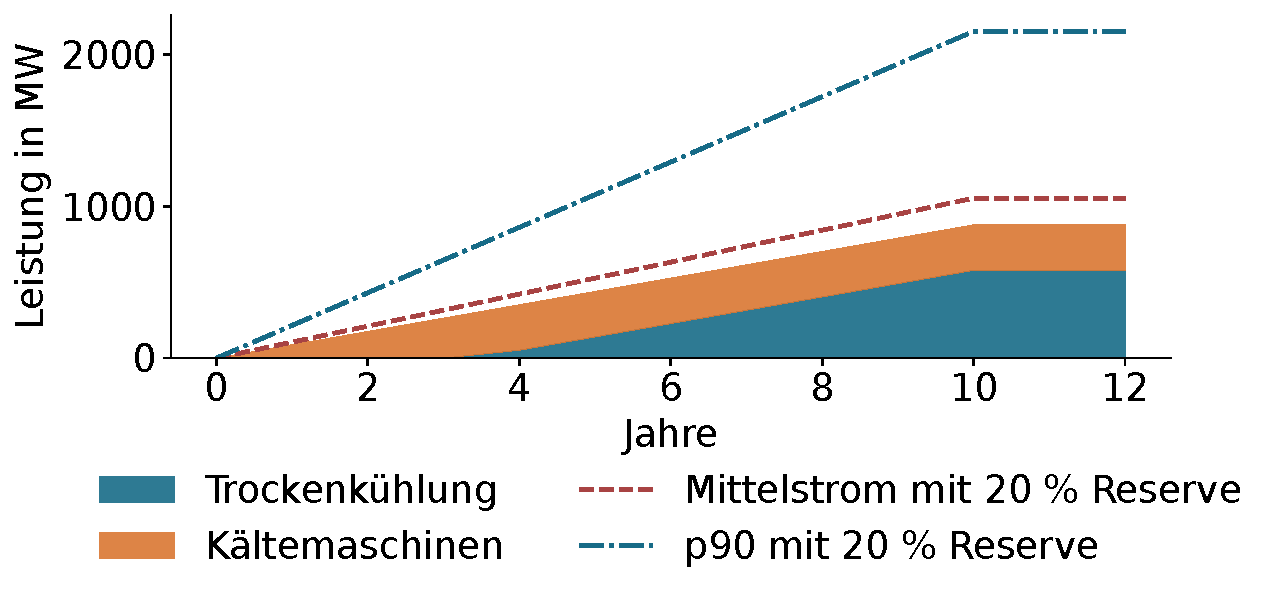
\includegraphics[width=\textwidth]{figures/fig02_stufenplan.pdf}
\caption{Abbildung 3 zeigt den modularen Ausbau. Die Trockenkühlung beginnt erst oberhalb ihrer treibenden Temperaturdifferenz. Die gestrichelte Linie enthält 20 \% Reserve. Eigene Rechnung mit Kimi K3.1 Pro.}
\label{fig:stufen}
\end{figure*}

\begin{figure*}[t]
\centering
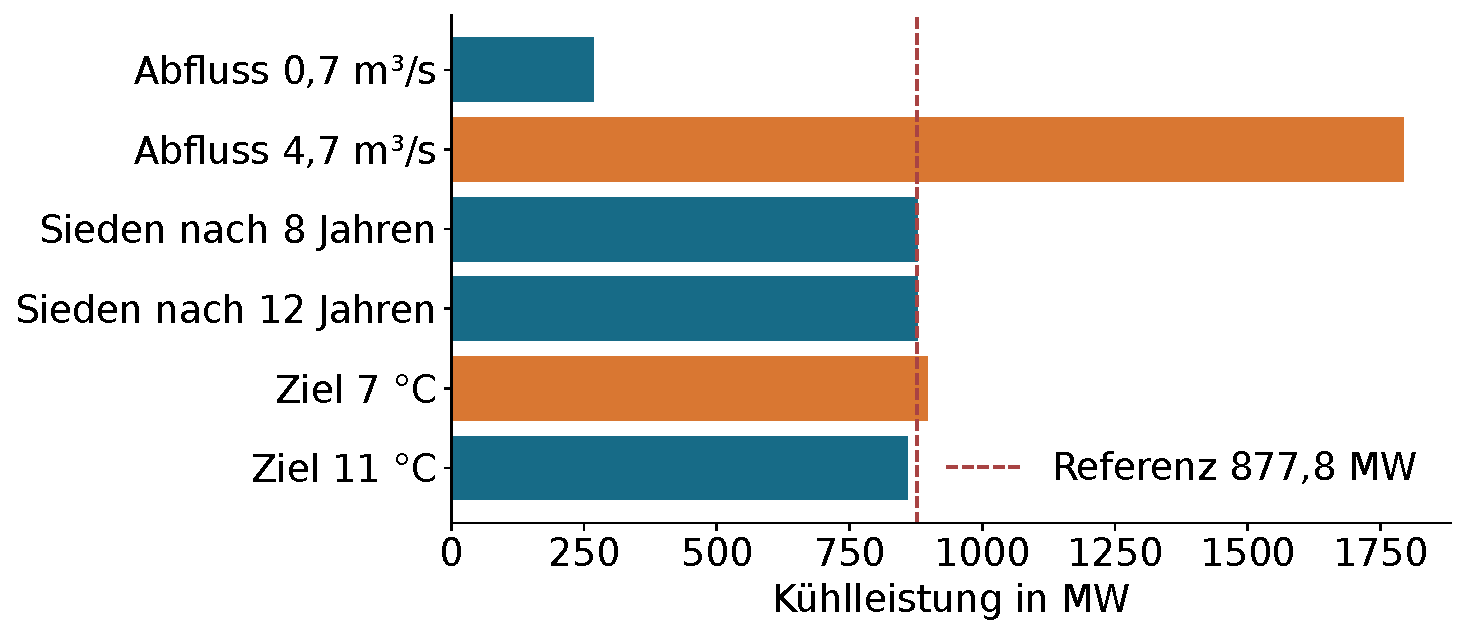
\includegraphics[width=\textwidth]{figures/fig04_sensitivitaet.pdf}
\caption{Abbildung 4 zeigt die Sensitivität gegenüber Abfluss, Prognosezeit und Rückführziel. Eigene Rechnung mit Kimi K3.1 Pro.}
\label{fig:sensitivitaet}
\end{figure*}

\begin{figure*}[t]
\centering
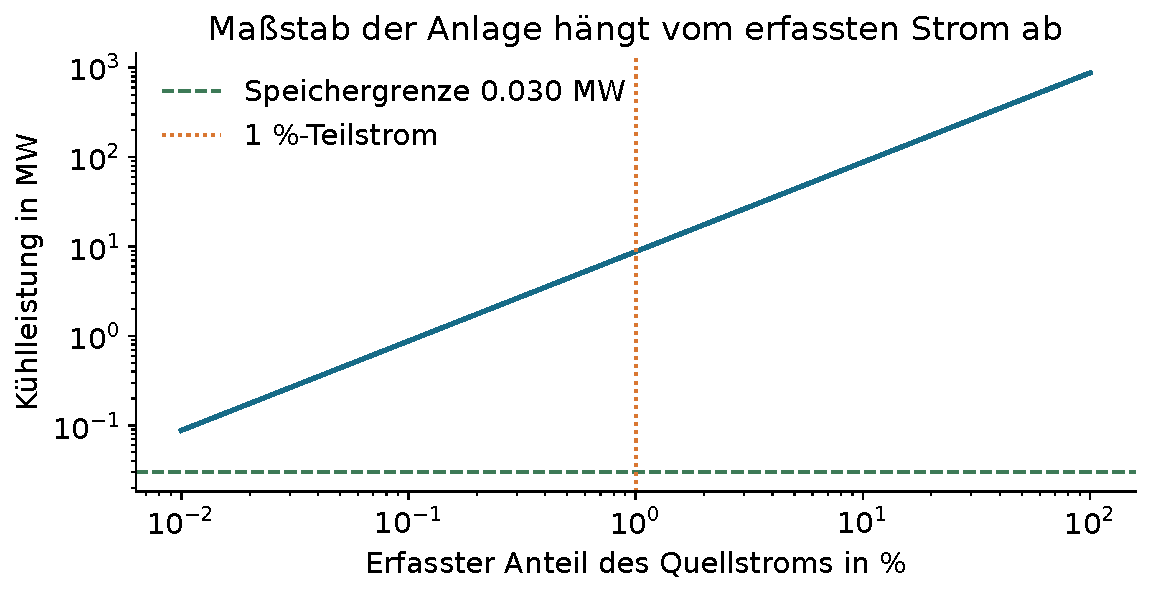
\includegraphics[width=\textwidth]{figures/fig06_teilstrom.pdf}
\caption{Abbildung 5 stellt Vollstrom, Teilstrom und isolierte Speichergrenze gegenüber. Eigene Rechnung mit Kimi K3.1 Pro.}
\label{fig:teilstrom}
\end{figure*}

\begin{figure*}[t]
\centering
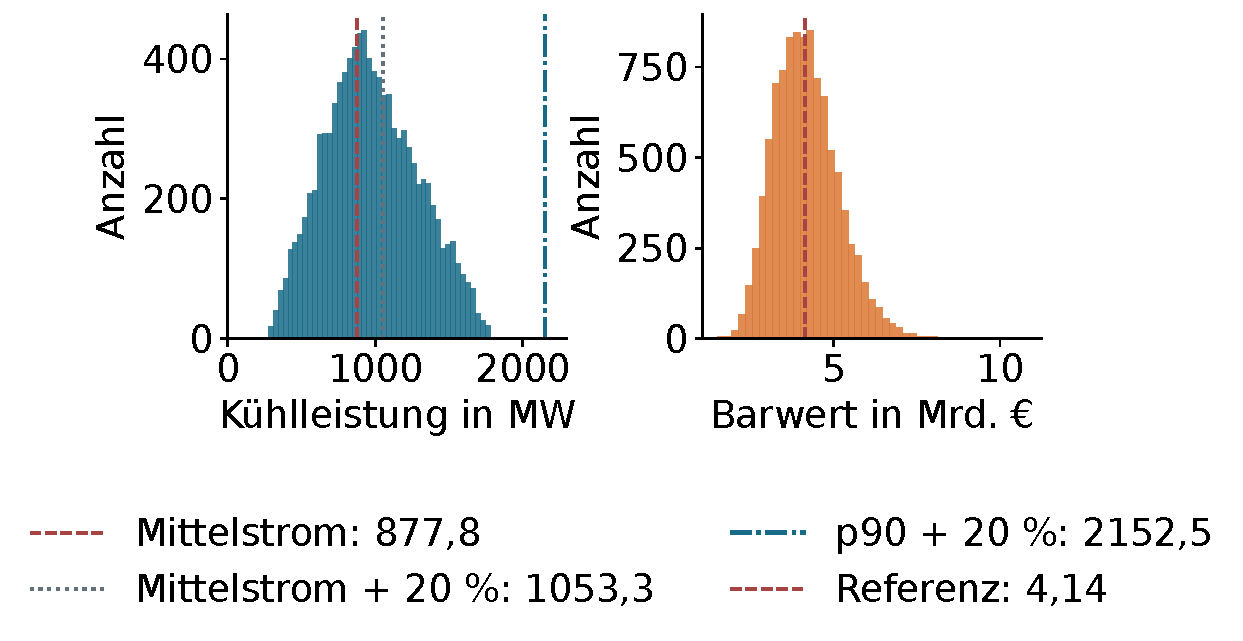
\includegraphics[width=\textwidth]{figures/fig05_unsicherheit.pdf}
\caption{Abbildung 6 zeigt die angenommenen Verteilungen für Abfluss, COP und Investitionskosten. Sie beschreiben Rechenunsicherheit, keine Vulkanwahrscheinlichkeit. Eigene Rechnung mit Kimi K3.1 Pro.}
\label{fig:unsicherheit}
\end{figure*}

\end{document}
